%\documentclass[11pt]{article}
\documentclass[a4paper,11pt]{article}
\usepackage{enumerate}%??item??????1??2???
\renewcommand{\labelitemi}{$\bullet$}%??item???-*??????
\usepackage{amsfonts,amssymb,amsmath,graphicx}
\usepackage{fullpage}
\begin{document}
\author{Zuodong Wu}
\title{CS653 Homework Two}
\maketitle
\section{Question 1}
\subsection{Part a}
\begin{description}
  \item [Solution]:

$$dC/dT=-\frac{C_rL}{T^2}+C_sP_s \triangleq 0$$
We get $$T^*=\sqrt{\frac{C_rL}{C_sP_s}}$$
\begin{eqnarray*} T^*= \begin{cases} \sqrt{\frac{C_rL}{C_s}}, &\mbox{soft state}\cr \sqrt{\frac{C_rL}{C_sp}}, &\mbox{hard state}\end{cases} \end{eqnarray*}
(It is easy to check that $\frac{d^2C}{dT^2}(T^*)>0$)
\end{description}
\subsection{Part b}
\begin{description}
  \item [Solution]:
  
  For a pure hard state protocol, $T^*=\sqrt{\frac{C_rL}{C_sp}}$, which is affected by $C_r$, $L$, and $C_s$, and:
  \begin{itemize}
  \item[$\bullet$] Hardness increases as $C_r$ and/or $L$ increase(s).
  \item[$\bullet$] Hardness decreases as $C_s$ and/or $p$ increase(s).
  \end{itemize}
  For a soft state protocol, $T^*=\sqrt{\frac{C_rL}{C_s}}$, which is affected by $C_r$, $L$, and $C_s$, and:
  \begin{itemize}
  \item[$\bullet$] Hardness increases as $C_r$ and/or $L$ increase(s).
  \item[$\bullet$] Hardness decreases as $C_s$ increases; Hardness does not be affected by $p$.
  \end{itemize}

\end{description}
\subsection{Part c}
\begin{description}
  \item [Solution]:
  
  \begin{eqnarray*} T^*= \begin{cases} \sqrt{\frac{1\times 10^4}{1}}=10^2, &\mbox{soft state}\cr  \sqrt{\frac{1\times 10^4}{1\times 10^{-4}}}=10^4, &\mbox{hard state}\end{cases} \end{eqnarray*}
  So,
  \begin{eqnarray*} C(T)= \begin{cases} 10^4/T^* + 10^4p + T^* =2\times 10^2 + 10^4p, &\mbox{soft state}\cr  10^4/T^* + 10^4p + pT^*=1+ 2\times 10^4p, &\mbox{hard state}\end{cases} \end{eqnarray*}
\begin{figure}[htbp]
\begin{center}
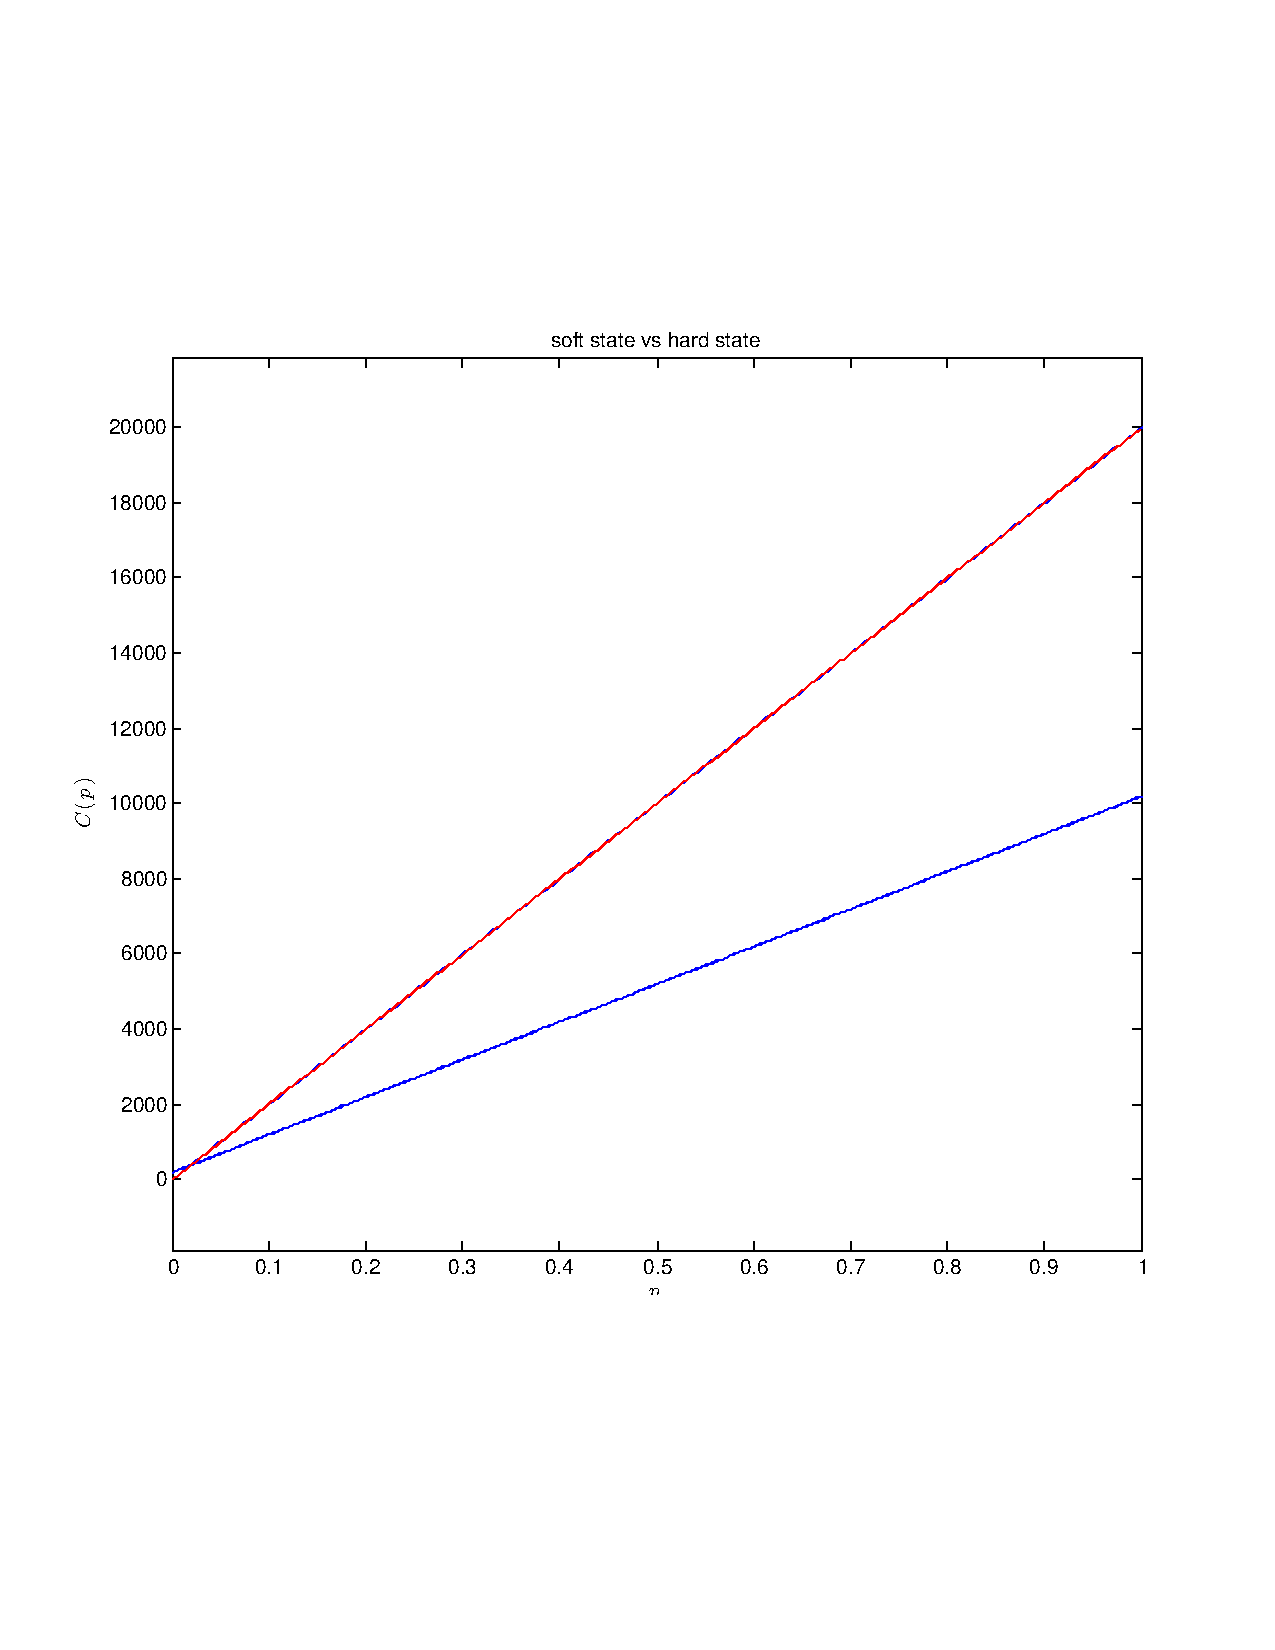
\includegraphics[width=0.6\textwidth]{./pdf/1.pdf}
\label{fig:3c1}
\caption{$C$ vs $p$}
\end{center}
\end{figure}
\end{description}
In the Figure 1, blue line corresponds with soft state scheme while red line corresponds with hard state. For low loss probability($p<0.02$), cost for hard state mechanism is smaller than soft state protocol, while for high loss probability($p>0.02$), cost for soft state mechanism is smaller. In my opinion, soft state protocol should be more robust, since the slope of the curve corresponding to the soft state mechanism is smaller (here it is just a half), which means the cost increases with a slower speed. Specifically, there are no orphan states for soft state protocol, which are caused by reasons like breakdown of a machine or a link.
\section{Question 2}
\subsection{Part a}
\begin{description}
  \item[Solution]:

I think it is because the TCP confronts a situation (the Internet) more complex than Ethernet, where the Internet has already introduced randomization to the TCP connection. 

Specifically, Ethernets are often deployed in a relative small space with at most a few hops of switches (e.g., in an office or an apartment), an interface would transmission from others almost immediately; at the situation, the latent collision would happen at the end hosts. In other words, each Ethernet interface can almost predict accurately when its sent frame would arrive at others; thus from the view of an Ethernet interface, it can be certain that the possibility to collide would be small if other interfaces choose the same randomization scheme (the Binary Exponential Backoff Scheme) as itself.

However, with regard to TCP, "Exponential Backoff" scheme is used in set Retransmission TimeOuts (RTOs), but it does not involve in randomization (As least for the current implementation of RTOs in RFC2988). "collisions" in Ethernet correspond here to congestions in some point in a link. For example, considering congestion happens in a router shared by several TCP connections, which makes the transmissions of their segments timeouts. Because it is hardly to predict when a retransmit segment from an end host would arrive at the point of congestion: the time is changing due to ceaselessly changing of the connection between the end host and the congestion point, e.g., increased offload of a router within the connection would enlarge the wait time of the retransmit segment, thus increasing the total transmission time. Such variance of transmission time is unpredictable and randomized from the whole system's view. Thus it is meaningless to add the randomization again, since the system has already done it for you.
\end{description}
\subsection{Part b}
\begin{description}
\item[Solution]:

Yes, I think TCP's timeout mechanism allow TCP to spread transmissions over longer periods of time (adaptively) as in Ethernet.

Firstly, TCP's timeout mechanism allow TCP to spread transmissions over long periods of time, since each time a transmission is timeout, the RTO will be doubled. If we assume the underlying structure of TCP connections are working normally (no broken links, no failed routers), at a given time (interval), there should always be segments and their ACKs (which are encapsulated in IP packets of network layer) served successfully through the whole connection, thus making the transmission successful; while transmissions of remaining segments timeout, and are delayed. Since the RTOs are doubled confronting every time, and the upper bound is suggested by RFC2988 as "A maximum value MAY be placed on RTO provided it is at least \emph{60 seconds}", which is a long period of time.

Secondly, it is much longer than Ethernet, since the largest timeout for the Ethernet to resend a frame is 1023 � 51.2?s which is even far shorter than a second.
\end{description}
\section{Question 3}
\subsection{Part a}
\begin{description}
  \item[Solution]:

In situations an user directly communicate to a remote the server, it is easy for an eavesdropper or some authorized user (like the administrator of the server) to access the user's information, and infringes his/her privacy, even though \emph{encryption} is used. "A web server can record the
Internet addresses at which its clients reside, and the times and frequencies of accesses by its clients. With additional effort, this information can be combined with other data to invade the privacy of clients
even further". So it is important to keep the user anonymous.

The randomization and indirection is used in the paper to achieve the anonymity of users when they communicate with remote server(s) and help protect their privacy in a much safer way. In particular, the paper uses blending for realizing anonymity, and indirection is the base for blending by introducing other users to form a crowd. Randomization is then used to (try to) make it impossible to distinguish action of originating requests with action of just forwarding.
\end{description}
\subsection{Part a}
\begin{description}
\item[Solution]:

I will take the \emph{Binary Exponential Backoff} mechanism in CSMA/CD as the example of randomization, and \emph{Internet Indirection Infrastructure} as the example of indirection.
\begin{description}
\item[1] \emph{Crowds} vs \emph{Binary Exponential Backoff} with respect to \emph{randomization}

Similarities
\begin{itemize}
\item[$\bullet$] Randomization for the two schemes are both subject to a uniform distribution.
\item[$\bullet$] Different instances (\emph{Ethernet Interface} vs \emph{users in a Crowd}) make decisions independently.
\end{itemize}
Differences
\begin{itemize}
\item[$\bullet$] They are used for solving different sort of problem (\emph{Solving Conflicts} vs \emph{Adding Anonymity}).
\item[$\bullet$] There are two steps in randomization of \emph{Crowds}. Before choosing which user to forward, the \emph{jondo} instance flips a biased coin to determine whether to forward to another \emph{jondo} instance, or to send directly to the server.
\item[$\bullet$] \emph{Binary Exponential Backoff} scheme is dynamic, with changing parameter of the uniform distribution (Interval doubles each failure), while no similar dynamics exist or described in \emph{Crowds}.
\end{itemize}
\item[2] \emph{Crowds} vs \emph{Internet Indirection Infrastructure} with respect to \emph{indirection}

Similarities
\begin{itemize}
\item[$\bullet$] Both utilize and implement specific schemes on additional node(s) other than sender and receivers.
\item[$\bullet$] Senders do not know receivers for both cases.
\end{itemize}
Differences
\begin{itemize}
\item[$\bullet$] Senders in crowds knows the receivers, while for $i3$, senders and crowds do not know each other (totally decoupled). 
\item[$\bullet$] For \emph{i3}, both sender (sending data actively) and receiver (adding trigger) need to communicate with the \emph{i3} node (the node which implements the indirection, in the similar place with members other then the sender in a crowd), while only receiver (sending request) is required to communicate with other members in its joined crowd.
\item[$\bullet$] Normally, there is a dedicated \emph{i3} server for a specific sender for all sending data.
\end{itemize}
\end{description}
\end{description}
\section{Question 4}
\begin{description}
  \item[Solution]:
  
    $b_i$ is the bucket size, while $r_i$ is the leak rate (with respect to packets, assuming that all packets have the same size for simplicity).
    \begin{description}
    \item[When $r_2 \geqslant r_1$]: 
    
    the 2nd leak bucket would always be empty, so over interval of length $t$: number of packets admitted less than or equal to $(r_1 t + b_1)$. Thus the equivalent single leak bucket satisfies:
    \begin{align*}
    r_3		& = r_1 \\
    b_3		& = b_1
    \end{align*}
    \item[When $r_2 < r_1$]: 
    
    The extreme case is the 1st and 2nd leak buckets are filled simultaneously, which means number of packets admitted less than or equal to $(r_2 t + b_1 + b_2)$. Thus the equivalent single leak bucket satisfies:
    \begin{align*}
    r_3		& = r_2 \\
    b_3		& = b_1 + b_2
    \end{align*}
    \item[In Summary]
    \begin{align*}
    r_3		& = \min(r_1,r_2) \\
    b_3		& = \begin{cases}b_1, & r_2\geqslant r_1 \\ b_1+b_2, & r_2< r_1\end{cases}
    \end{align*}
    \end{description}
\end{description}
\end{document}

\section{Question 4}
\begin{description}
  \item[Solution]:
  
    $b_i$ is the bucket size, while $r_i$ is the leak rate (with respect to packets, assuming that all packets have the same size for simplicity).
    \begin{description}
    \item[When $r_2 \geqslant r_1$]: 
    
    the 2nd leak bucket would always be empty, so over interval of length $t$: number of packets admitted less than or equal to $(r_1 t + b_1)$. Thus the equivalent single leak bucket satisfies:
    \begin{align*}
    r_3		& = r_1 \\
    b_3		& = b_1
    \end{align*}
    \item[When $r_2 < r_1$]: 
    
    The extreme case is the 1st and 2nd leak buckets are filled simultaneously, which means number of packets admitted less than or equal to $(r_2 t + b_1 + b_2)$. Thus the equivalent single leak bucket satisfies:
    \begin{align*}
    r_3		& = r_2 \\
    b_3		& = b_1 + b_2
    \end{align*}
    \item[In Summary]
    \begin{align*}
    r_3		& = \min(r_1,r_2) \\
    b_3		& = \begin{cases}b_1, & r_2\geqslant r_1 \\ b_1+b_2, & r_2< r_1\end{cases}
    \end{align*}
    \end{description}
\end{description}
\end{document}













